
%=========================================================
\begin{figure*}[t]
\centering
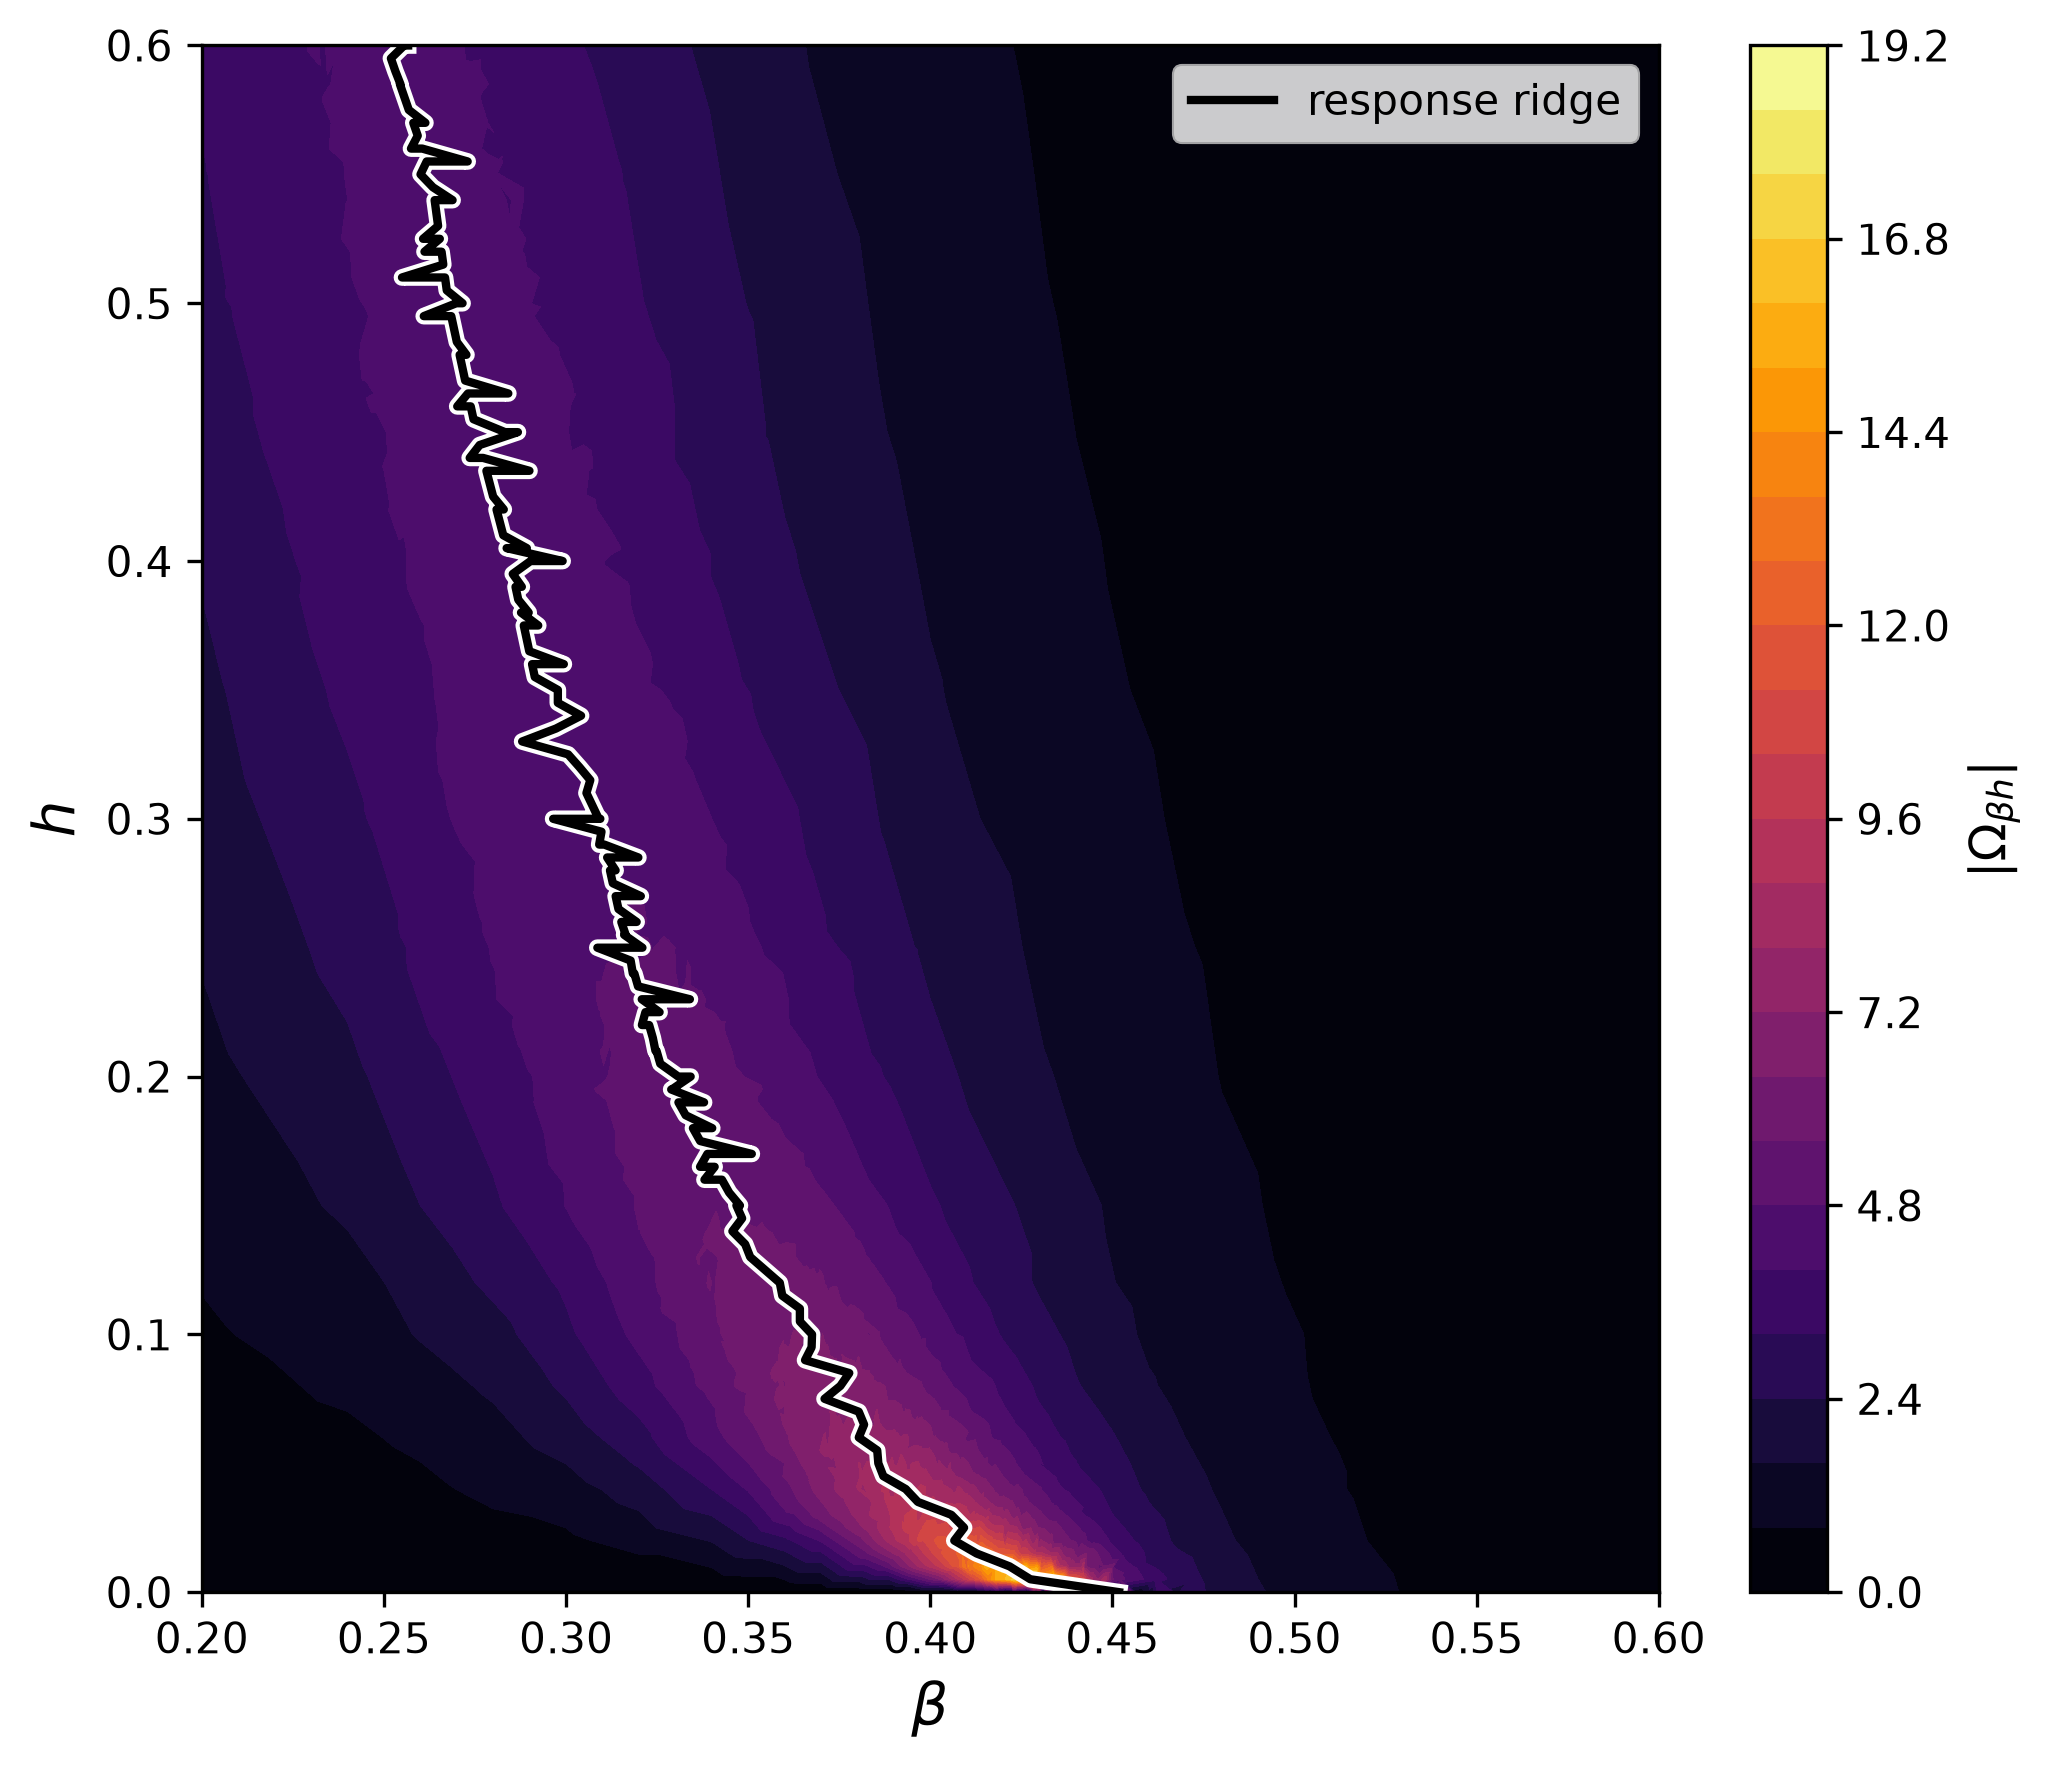
\includegraphics[width=0.85\textwidth]{Figures/ising_curvature_field_Omega.png}
\caption{
Mixed-response landscape
\(\Omega_{Th}(T,h)\)
for the two-dimensional Ising model together with the
extracted loci of maximal response.
The color scale indicates the magnitude of the mixed
fluctuation field, while the superimposed curves denote ridge
trajectories obtained from maxima of the response functions.
Unlike conventional phase diagrams, which classify equilibrium
states, the present construction characterizes how those
states respond to perturbations. The mixed-response ridge
extends well beyond the Onsager critical point into the
supercritical regime, revealing an extended pathway along
which thermal and magnetic fluctuations remain maximally
coupled. The existence of multiple ridge trajectories
associated with different response sectors demonstrates that
the supercritical region is organized by a hierarchy of
response structures rather than a single universal crossover
curve.
}
\label{fig:ising_ridge}
\end{figure*}
%=========================================================
